\documentclass[12pt]{article}
\usepackage{graphicx}
\usepackage{caption}
\usepackage{placeins}
\usepackage{amsmath}
\begin{document}
\begin{titlepage}
\begin{center}
	\textsc{\LARGE Rutgers University}\\[1.5 cm]
    \textsc{\Large Physics 2 lab}\\[0.5cm]
    \rule{\linewidth}{0.5mm} \\ [.4 cm]
    {\huge \bfseries Magnetic Fields}\\[.4 cm]
    \rule{\linewidth}{0.5mm} \\ [1.5 cm]
    \begin{minipage}{0.4\textwidth}
	\begin{flushleft} \large
	\emph{Authors:}\\
	Brittney,Kishan,Abhi
	\end{flushleft}
	\end{minipage}
	\begin{minipage}{0.4\textwidth}
	\begin{flushright} \large
	\emph{Teacher:} \\
	James
	\end{flushright}
	\end{minipage}\\[2 cm]
	\textsc{ \Large Signatures} \\[1.7 cm] 
	\rule{10 cm}{0.5mm} \\ [2.0 cm]
	\rule{10 cm}{0.5mm} \\ [2.0 cm]
	\rule{10 cm}{0.5mm}
	\vfill
	{\large {July 31, 2013}}
\end{center}
\end{titlepage}

\section*{Part 1 -  Magnetic Field around a straight wire}
\subsection*{procedure and goal}

We set up a power source, ammeter, and straight wire in series. We had a probe which could measure the magnetic field at any point in space.We completed two different experiments. In the first experiment we measured the magnetic field strength around the straight wire with a fixed distance but varying current.In the second experiment we measured the magnetic field strength around the straight wire with a fixed current but varying distance. Our goal was to find the relationship between magnetic field to distance, as well as magnetic field to current.

\subsection*{results}
	
	\begin{table}[hp]
	\caption{With a fixed distance}
	\centering
	\begin{tabular}{|r|r|}
	\hline 
	I(amperes) & B(Gauss) \\
	\hline 
	0.00 & .041 \\
	1.00 & .168 \\
	1.23 & .217 \\
	1.51 & .254 \\
	2.03 & .320 \\
	2.23 & .336 \\
	2.60 & .369 \\
	\hline
	\end{tabular}
	\end{table}

	\begin{table}[hp] 
	\caption{With fixed current}
	\centering
	\begin{tabular}{|r|r|r|}
	\hline 
	N(turns) & B(Gauss) & 1/B(Gauss) \\
	\hline 
	0 & .318 & 3.144 \\
	2 & .296 & 3.37 \\
	4 & .283 & 3.53 \\
	6 & .244 & 4.09\\
	8 & .223 & 4.48 \\
	10 & .211 & 4.73 \\
	12 & .188  & 5.31\\
	\hline
	\end{tabular}
	\end{table}

	\begin{figure}[hp]
	 \centering
	 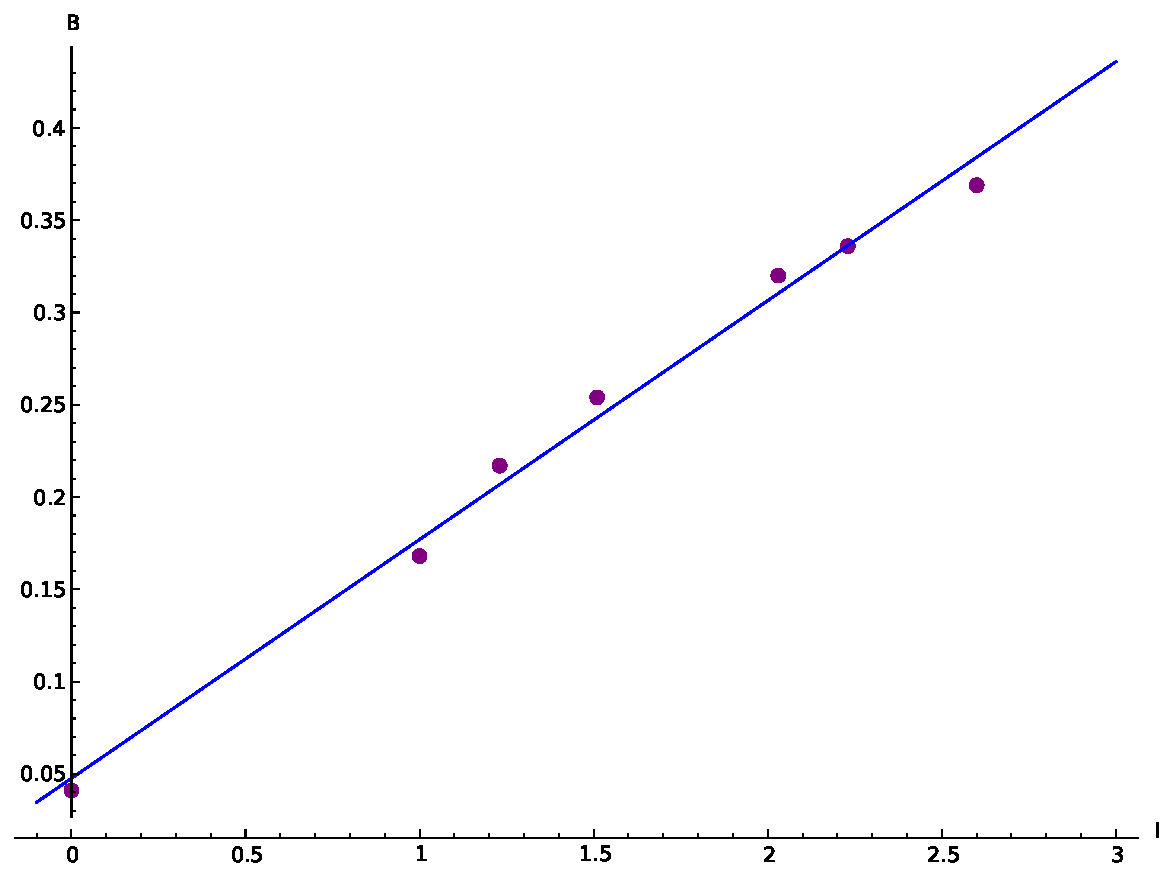
\includegraphics[scale = .85]{plot1}
	 \caption*{table 1 data: $I$ vs $B$. Best fit line is $B = .129I + .047$}
	\end{figure} 

	\begin{figure}[hp]
	 \centering
	 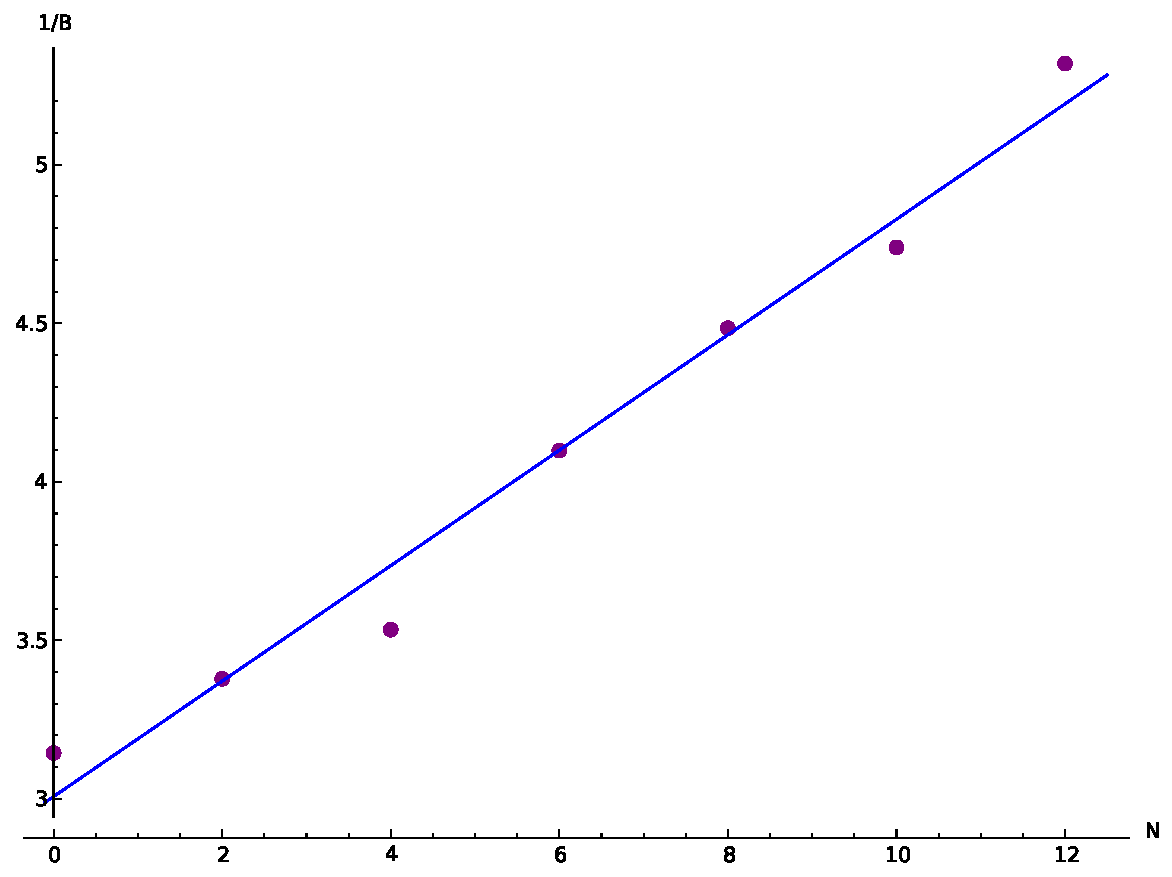
\includegraphics[scale = .85]{plot2}
	 \caption*{table 2 data: $N$ vs $\frac{1}{B}$. Best fit Line is $ \frac{1}{B} = .18N + 3 $}
	\end{figure}
	\FloatBarrier

\subsection*{analysis}
In graph 1, we noticed that there is a linear relationship between the magnetic field strength and the current. The best fit curve was $B=.129I+.047$. In graph 2, we found there is  a linear relationship between $\frac{1}{B}$ and $N$(number of turns). The best fit curve was $1/B=.18N+3$.



\section*{part 2 - Magnetic Field around Magnet}

\subsection*{procedure and goal}

We used the same probe as in part 1 to measure the magnetic field. This time we measured the magnetic field around a magnet instead a wire. We measured the magnetic field at varying distances. Our goal was to find the relationship between magnetic field strength and distance from the magnet.  

\subsection*{results} 
	\begin{table}[h]
	\caption{}
	\centering
	\begin{tabular}{|r|r|r|}
	\hline 
	D(cm) & B(Gauss) & 1/B(Gauss) \\
	\hline 
	2.5 & 1.41 & .709 \\
	3.5 & 1.21 & .826 \\
	4.5 & .914 & 1.09 \\
	5.5 & .274 & 3.64 \\
	6.5 & .07 & 14.28 \\
	\hline
	\end{tabular}
	\end{table}

	\begin{figure}[hp]
	 \centering
	 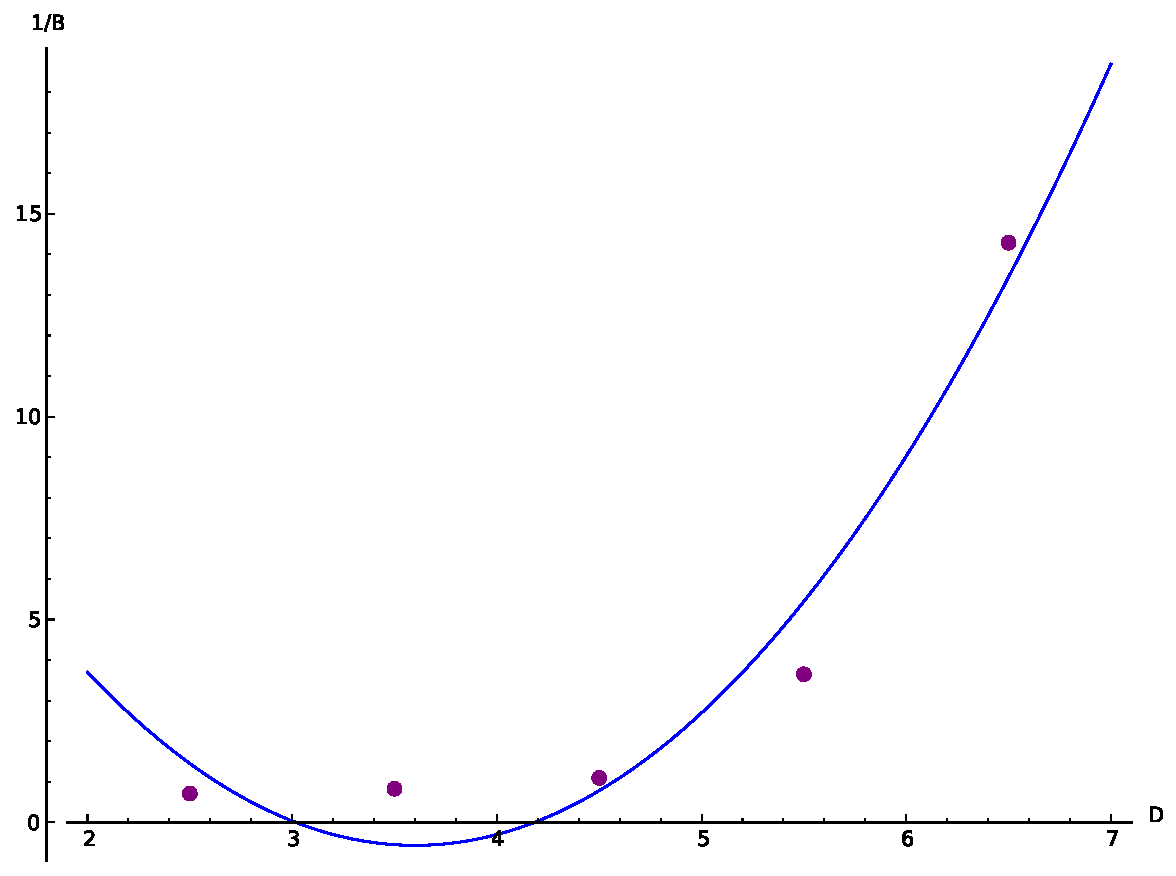
\includegraphics[scale = .85]{plot3}
	 \caption*{table 3 data: $D$ vs $\frac{1}{B}$. Best fit quadratic was $ \frac{1}{B} = 1.66D^2  - 11.99D + 21.03 $}
	\end{figure} 

	\begin{figure}[hp]
	 \centering
	 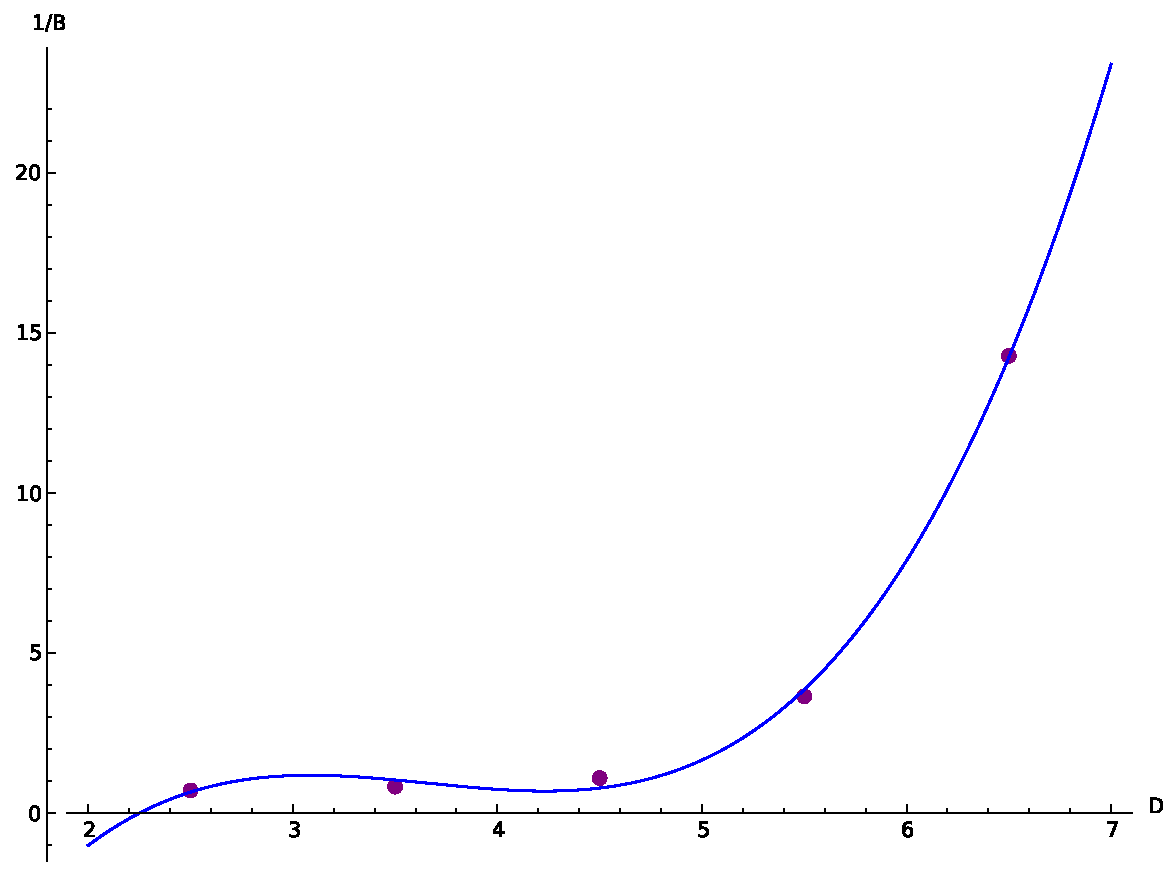
\includegraphics[scale = .85]{plot4}
	 \caption*{table 4 data: $D$ vs $\frac{1}{B}$. Best fit cubic was $ \frac{1}{B} = .066D^3  - 7.25D^2 + 25.9D - 29.07 $}
	\end{figure} 
	\FloatBarrier

\subsection*{analysis}
 We were able to see that the magnetic field gets weaker as you get farther from the magnet. But it is not clear what the best fit curve is. We only had 5 data points to work with so the cubic was obliviously the best fit.The best fit curve was  ($\frac{1}{B} = .066D^3  - 7.25D^2 + 25.9D - 29.07$).But with more points it is possible the the correct relationship is the quadratic.    

\end{document}
